\documentclass{SimSemBericht} % Eigene Klasse für Formatierung

% ----- Zusätzliche Pakete, falls benötigt -----
% (Die meisten Pakete und Einstellungen sind bereits in SimSemBericht.cls enthalten)
% \usepackage{enumitem}          % Falls spezielle Aufzählungen benötigt werden
% \usepackage{xcolor}            % Für zusätzliche Farben im Text

% ----- Titel -----
\title{Simulation einer Wasserrakete}
\author{Simon Kerlin, Patrick Stempel \\[0.5em]
Betreuer: Prof. Dr. Peter Jonas}
\date{\today} % Optional

% ==========================
\begin{document}
% ==========================

\maketitle % Titel ausgeben

\tableofcontents % Inhaltsverzeichnis
\newpage

\section{Funktionsweise einer Wasserrakete}
Der Körper einer Wasserrakete besteht typischerweise aus einer stabilen Kunststoffflasche (z.B. 1 Liter Fanta-Flasche), die teilweise mit Wasser gefüllt wird (siehe Abbildung~\ref{fig:wasserrakete}). 
Anschließend wird die übrige Luft in der Flasche unter Druck gesetzt.
Die Flasche dient als Druckbehälter und gleichzeitig als Raketenkörper.

\begin{figure}[h!]
    \centering
    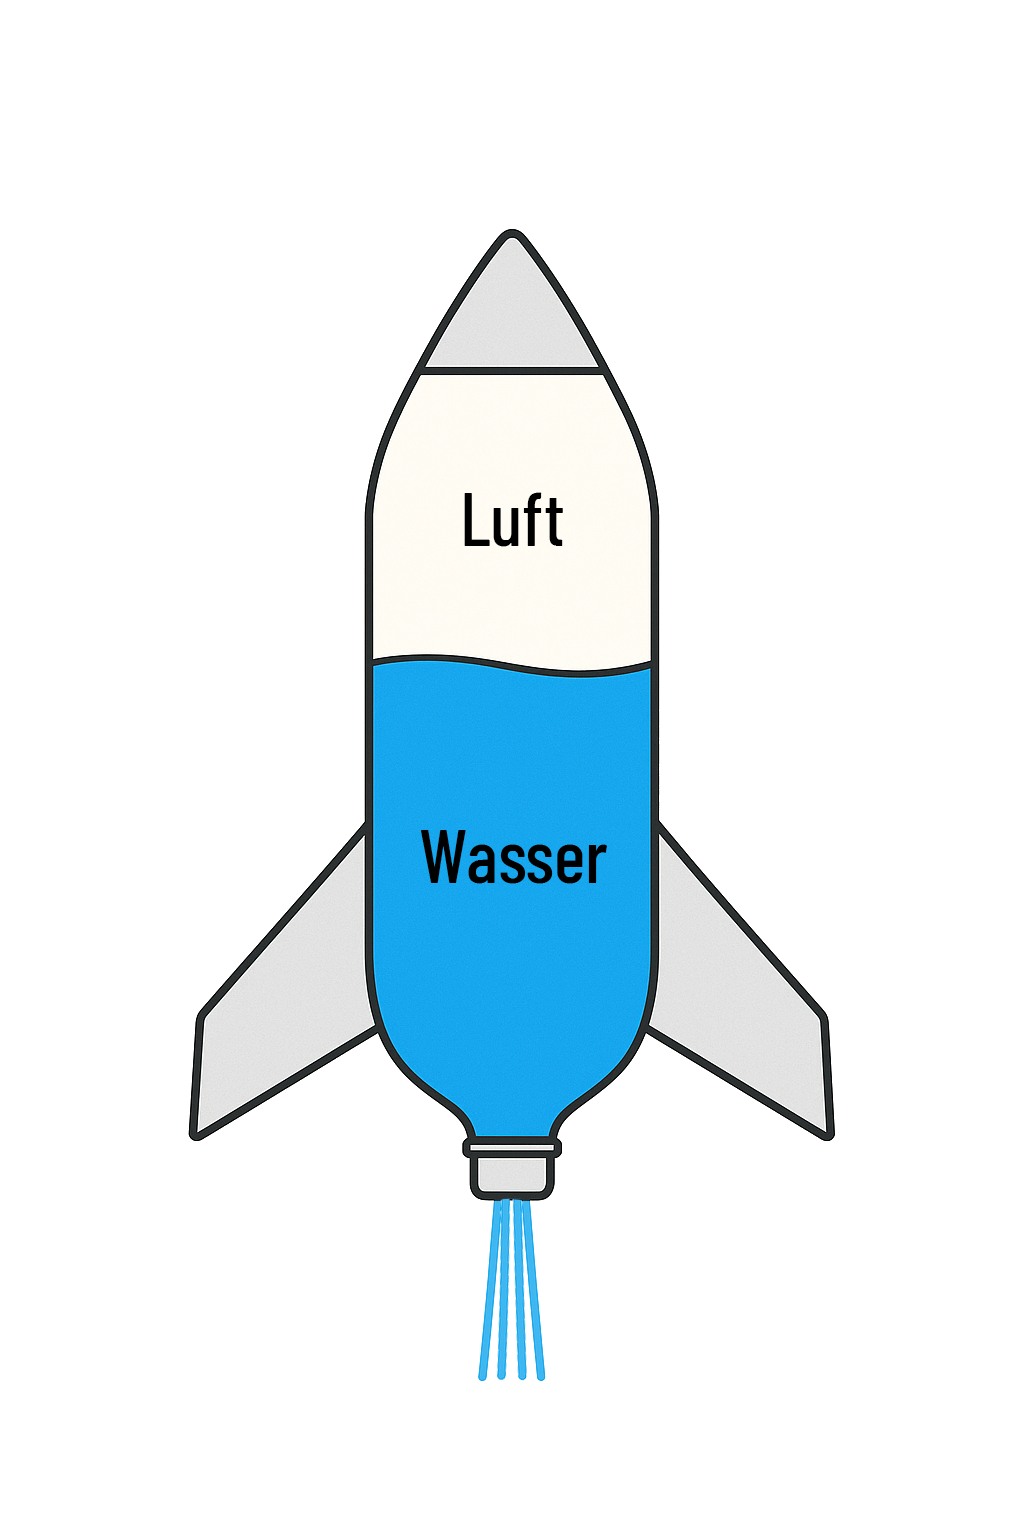
\includegraphics[width=0.5\textwidth]{wasserrakete_schematisch.png}
    \caption{Schematischer Aufbau einer Wasserrakete.}
    \label{fig:wasserrakete}
\end{figure}

\textcolor{red}{Ablauf des Starts (muss noch geprüft werden):}
\newline
\textcolor{lightgray}{Vor dem Start wird die Rakete auf eine Startrampe gesetzt und mit einer Düse verschlossen. Über ein Ventil wird Luft in die Flasche gepumpt, wodurch sich der Druck im Inneren erhöht. Das Wasser fungiert als Reaktionsmasse.}
\textcolor{lightgray}{Beim Auslösen des Starts öffnet sich die Düse, und das unter Druck stehende Wasser wird mit hoher Geschwindigkeit nach hinten ausgestoßen. Nach dem Rückstoßprinzip (3. Newtonsches Gesetz) erfährt die Rakete eine entgegengesetzte Beschleunigung und hebt ab.}

Die Flugbahn der Rakete wird durch verschiedene Faktoren beeinflusst:
\begin{itemize}
    \item Leergewicht der Rakete
    \item Füllmenge des Wassers
    \item Luftdruck im Inneren
    \item Düsengröße
    \item Aerodynamik des Raketenkörpers
\end{itemize}

Nachdem das gesamte Wasser ausgestoßen ist, fliegt die Rakete im freien Fall weiter, bis sie schließlich wieder am Boden aufschlägt. 
Ein Fallschirm kann zur sicheren Landung beitragen, diesen haben wir jedoch nicht in unsere Simulation integriert.

\section{Mathematisch-Physikalisches Modell}
Die Bewegung der Wasserrakete wird durch verschiedene physikalische Prozesse bestimmt. 
Wir haben uns bewusst für ein vereinfachtes Modell entschieden, das die wesentlichen Aspekte des Raketenflugs erfasst, ohne zu komplex zu werden. 
Beispielsweise werden Effekte wie Turbulenzen und komplexe Strömungsdynamiken vernachlässigt.
Im Folgenden werden die Gleichungen aufgeführt, die in unserem Modell verwendet werden.

\subsection{Druckentwicklung}
Das Volumen der Luft in der Flasche ändert sich während des Ausstoßes des Wassers, wofür zwei verschieden Gleichungen in Frage kommen:

\begin{itemize}   
    \item Die isotherme Zustandsänderung (\(\Delta T = 0\)):
    \begin{equation}p_0 V_0 = p_1 V_1\end{equation}
    \item und die adiabatische Zustandsänderung (\(\Delta Q = 0\)) :
    \begin{equation}
        p_0 V_0^\kappa = p_1 V_1^\kappa
        \label{eq:adiabatisch}
    \end{equation}
\end{itemize}
Wir haben uns für die adiabatische Zustandsänderung~\eqref{eq:adiabatisch} entschieden, da der Druckabfall in der kurzen Zeit des Ausstoßes schneller erfolgt als der Wärmeaustausch mit der Umgebung.
Dabei ist $p_0$ der Anfangsdruck, $V_0$ das Anfangsvolumen der Luft, $p_1$ bzw. $V_1$ die Größen nach der Expansion und $\kappa$ der Adiabatenexponent (für Luft $\kappa \approx 1{,}4$).

\subsection{Ausstoßgeschwindigkeit des Wassers}
Die Geschwindigkeit \(v_\text{A}\), mit der das Wasser durch die Düse ausgestoßen wird, ergibt sich aus der Bernoulli-Gleichung:
\begin{equation}
    p - p_\text{atm} = \frac{1}{2} \rho_\text{Wasser} \cdot v_\text{A}^2
\end{equation}
Umgestellt nach \(v_\text{A}\) ergibt sich:
\begin{equation}
v_\text{A} = \sqrt{ \frac{2 (p - p_\text{atm})}{\rho_\text{Wasser}} }
\end{equation}
$p$ ist der Druck in der Flasche, $p_\text{atm}$ der Umgebungsdruck und $\rho_\text{Wasser}$ die Dichte des Wassers.

\subsection{Massenstrom}
Der Massenstrom \(\dot{m}\) des ausgestoßenen Wassers berechnet sich aus der Kontinuitätsgleichung:
\begin{equation}
\dot{m} = \rho_\text{Wasser} \cdot v_\text{A} \cdot A_\text{Düse}
\end{equation}
$A_\text{Düse}$ ist die Querschnittsfläche der Düse.

\subsection{Schubkraft}
Die Schubkraft \(F_\text{Schub}\), die auf die Rakete wirkt, ist:
\begin{equation}
F_\text{Schub} = \dot{m} \cdot v_\text{A}
\end{equation}

\subsection{Kräftebilanz}
Die Rakete erfährt neben dem Schub auch Luftwiderstand und Gewichtskraft:
\begin{equation}
F_\text{gesamt} = F_\text{Schub} - F_\text{Luftwiderstand} - F_\text{G}
\end{equation}
Der Luftwiderstand wird mit folgender Formel abgeschätzt:
\begin{equation}
F_\text{Luftwiderstand} = \frac{1}{2} C_w \cdot \rho_\text{Luft} \cdot A_\text{Quer} \cdot v^2
\end{equation}
Dabei ist \(C_w\) der Luftwiderstandsbeiwert (Annahme: \(C_w \approx 1\)), \(\rho_\text{Luft}\) die Dichte der Luft, \(A_\text{Quer}\) die Querschnittsfläche der Rakete senkrecht zur Flugrichtung und \(v\) die Geschwindigkeit der Rakete.

\subsection{Bewegungsgleichungen}
Die Bewegungsgleichungen für die Rakete lauten:
\begin{equation}
a = \frac{F_\text{gesamt}}{m_\text{Rakete}}
\end{equation}
\begin{equation}
    v = \int a(t) \, dt
\end{equation}
\begin{equation}
    h = \int v(t) \, dt
\end{equation}

\section{Implementierung des Modells}
\subsection{Numerische Methoden}
\subsection{Aufbau des Programms}

\section{Benutzerhandbuch für das Programm}
Erklärung der GUI und der verschiedenen Buttons
\section{Simulationsergebnisse}
Um die Simulationsergebnisse auswerten zu können, mussten wir uns zuerst überlegen, an welcher Stelle der Rakete wir die Höhe messen. Zur Entscheidung standen:
\begin{itemize}
    \item Spitze der Rakete
    \item Schwerpunkt der Rakete
    \item Boden der Rakete
\end{itemize}
Obwohl vermutlich der Schwerpunkt der Rakete die gebräuchlichste Wahl ist, haben wir uns für den Boden der Rakete entschieden, da sich der Schwerpunkt der Rakete während des Fluges durch das Ausstoßen des Wassers kontinuierlich ändert.
\subsection{Maximale Höhe und Auftreffgeschwindigkeit}
\subsection{Optimaler Füllstand und Düsengröße}

\subsection{Vergleich mit der Realität}

\section{Diskussion}
Folgeuntersuchungen, Schwachstellen des Modells
(z.B keine Turbulenzen, kein Wind, kein Fallschirm, Abschusswinkel nur 90°, etc.)

\section{Bilder}
\begin{figure}[h!]
    \centering
    % \includegraphics[width=0.5\textwidth]{beispielbild.png}
    \caption{Ein Beispielbild.}
    \label{fig:beispiel}
\end{figure}


% ==========================
\end{document}
% ==========================
